%\documentclass[a4paper,10pt]{article}
\documentclass[10pt, conference, letterpaper]{IEEEtran}
\usepackage[utf8]{inputenc}
\usepackage{xspace}
\usepackage{url}
\usepackage{graphicx,graphics} 
\usepackage{color}
\usepackage{amsmath}
\usepackage{amsfonts}
\usepackage{amssymb}
\usepackage{amsthm}
\usepackage{algorithm}
\usepackage{algorithmic}
\usepackage{longtable}
\usepackage{complexity}
\usepackage{tkz-graph}
\usepackage{float}
\usepackage{tabularx}
\usepackage{setspace}
\usepackage{icomma}
\renewcommand{\algorithmicrequire}{\textbf{Input:}}
\renewcommand{\algorithmicensure}{\textbf{Output:}}
\usepackage{authblk}
\usepackage[colorlinks=true,breaklinks=true,linkcolor=blue]{hyperref}

    
\graphicspath{{figures/}}
\makeatletter
\def\input@path{{figures/}}
\makeatother
\newcommand\rmatching{${\cal R}$-matching\xspace}
\newcommand\mdelay{$\cal M$-delay\xspace}
\newcommand\matchedgraph{{\bf matched graph}}
\newtheorem{proposition}{Proposition}
\newtheorem{theorem}{Theorem}

\setlength{\parskip}{1ex} % Espace entre les paragraphes

\newtheorem{fact}{Fact}
\newtheorem{lemma}[theorem]{Lemma}
\newtheorem{definition}{Definition}
\newtheorem{corollary}{Corollary}

% \renewcommand{\thefootnote}{\*}

\newcommand{\todo}[1]{{\color{red} TODO: {#1}}}
\newcommand\pazl{\textsc{pazl}\xspace}
\newcommand\pall{\textsc{pall}\xspace}
\newcommand\bra{\textsc{bra}\xspace}
%opening
\title{Deterministic Scheduling of Periodic Messages for Cloud RAN}
 

\author[1]{Dominique Barth}
\author[1]{Ma\"el Guiraud}
% \author[1]{Christian Cad\'er\'e}
\author[2]{Brice Leclerc}
\author[2]{Olivier Marc\'e}
\author[1]{Yann Strozecki}
\affil[1]{David Laboratory, UVSQ}
\affil[2]{Nokia Bell Labs France}

\begin{document}

\maketitle

\begin{abstract}
A recent trend in mobile networks is to centralize in distant data-centers the processing units which were attached to 
antennas until now. The main challenge is to guarantee that the latency of the periodic messages sent from the antennas to their processing
units and back, fulfills protocol time constraints. We show that traditional statistical multiplexing does not allow such a low latency, due to collisions and buffering at nodes. Hence, we propose in this article to use a deterministic scheme for sending periodic messages without collisions in the network thus saving the latency incurred by buffering.

We give several algorithms to compute such schemes for a common topology where one link is shared by all antennas.
We show that there is always a solution when the routes are short or the load is small. When the parameters are unconstrained,
and some buffering is allowed in the processing units, we propose an algorithm (PMLS) adapted from a classical scheduling method.
The experimental results show that even under full load, most of the time PMLS finds a deterministic sending scheme with no latency.
\end{abstract}


\section{Introduction}

Next generations of mobile network architectures evolve toward centralized radio network architectures called C-RAN for Cloud Radio Access Network, to reduce energy consumption costs~\cite{mobile2011c} and more generally the total cost of ownership. The main challenge for this type of architecture is to reach a latency compatible with transport protocols. The latency is measured between the sending of a message by a Remote Radio Head (RRH) and the receptions of the answer, computed by real-time virtualized network functions of a BaseBand Unit (BBU)\footnote{Others terminologies exist in the literature. The results of this work are fully compatible with any C-RAN architecture definition.} in the cloud. For example, LTE standards require to process functions like HARQ (Hybrid Automatic Repeat reQuest) in $3$ms~\cite{bouguen2012lte}. In 5G, some services need end-to-end latency as low as $1$ms~\cite{3gpp5g}. The specificity of the C-RAN context is not only the latency constraint, but also the periodicity of the data transfer in the \emph{frontaul} network between RRHs and BBUs: frames need to be emitted and received each millisecond~\cite{bouguen2012lte}.
Our aim is to operate a C-RAN on a low-cost shared switched network.
The question we address is the following: is it possible to schedule messages such that there are no collisions to avoid latency caused by queuing delays? 
Eliminating this source of latency leaves us with more time budget for latency due to the physical length of the routes in the network, and thus allows for wider deployment areas.


Let us expose briefly our model: the network topology is modeled by a directed weighted graph and a set of paths (routes) from source nodes (RRHs) to target nodes (BBUs). Time is discretized and a unit of time or slot corresponds to the time needed to transmit a minimal unit of data over the network. Since statistical multiplexing does not ensure a good latency we want to avoid any  buffering in internal nodes of the graph.  We take advantage of the deterministic nature of the messages we must manage i.e. the dates of arrival of messages are known beforehand. In fact, following LTE standard~\cite{bouguen2012lte}, we assume that the arrivals of all the packets are periodic with the same period. We propose to design a \emph{periodic} process to send the messages through the network without collisions. By periodic process we mean that the network at times $t$ and $t+P$ where $P$ is the period, is in the exact same state. 

We assume that the routes of the messages are already fixed, and there are no buffering allowed inside the network. Hence we only have two sets of values that we can set when building a periodic sending process, called a \emph{periodic assignment}: the time at which each packet is sent by an RRH in each period and the waiting time in the BBU before the answer is sent back to the RRH. When building a periodic assignment, we must take into account the periodicity which makes many scheduling methods unusable. Not only a message must not collide with the other messages sent by the others BBU/RRH in the same period, but also in the previous and following periods. The latency, that is the time between the emission of a message and the complete return of its answer must be minimized. This means that the only buffering we are allowed -- the waiting time before sending back the answer-- must be small, in particular when the route is long. Note that the model is technology agnostic, i.e. it is compatible with an optical network with a fixed packet size.   

Our main contributions are the following.
 In Sec.~\ref{sec:def} we propose a model of the network and the periodic sending of messages along its routes and we introduce the star routed network. We formalize the problem of finding a periodic assignment for sending messages without buffering (\pazl) or with buffering in the processing unit only (\pall). In Sec.~\ref{sec:PAZL}, we propose several algorithms to solving \pazl and evaluate their efficiency experimntally. Finally in Sec.~\ref{sec:PALL}, we introduce two algorithms to solve \pall and our experimentations show that the deterministic communication schemes we design vastly outperform the traditional statistical multiplexing with regard to latency. 
 
 \subsection*{Related works}

 Statistical multiplexing even with a large bandwidth does not comply with the latency requirements of C-RAN. Therefore, the current solution~\cite{pizzinat2015things,tayq2017real} is to use dedicated circuits for the fronthaul. Each end-point (RRH on one side, BBU on the other side) is connected through direct fiber or full optical switches. This architecture is very expensive and hardly scales in the case of a mobile network composed of about $10,000$ base stations. The deterministic approach we propose has gained some traction recently: Deterministic Networking is under standardization in IEEE 802.1 TSN group~\cite{finn-detnet-architecture-08}, as well at IETF DetNet working group~\cite{ieee802}. Several patents on concepts and mechanisms for DetNet have been already published, see for example~\cite{howe2005time,leclerc2016transmission}. 
     
The algorithmic problems we study are similar to several optimization problems: such as the allocation of frequencies~\cite{borndorfer1998frequency}, designing train schedules~\cite{strotmann2007railway} with small latency or the two flow shop scheduling problem~\cite{yu2004minimizing}. However, in our case the periodicity of our problems makes them significantly different.


\section{Model and Problems}\label{sec:def}

A long version of this paper~\cite{versionlongue} contains details on the models, hardness results, 
additional algorithms and proofs.  

  \subsection{Network modeling}
  

The network is modeled as a directed graph $G=(V,A)$. Each arc  $(u,v)$ in $A$ is labeled by an integer weight $\omega(u,v)$ which represents the time taken by a message to go from $u$ to $v$ using this arc. A {\bf route} $r$ in $G$ is a directed path, that is, a sequence of adjacent vertices $u_0, \ldots , u_{k}$, with $(u_i,u_{i+1}) \in A$.  The {\bf latency} of a vertex $u_i$ in a path $r$ is defined by $\lambda(u_i,r)= \sum\limits_{0 \leq j <i} \omega(u_j, u_{j+1})$. We also define $\lambda(u_0,r)=0$. The length of the route $r$ is defined by $\lambda (r)= \lambda (u_k,r)$.
We denote by $\cal R$ a set of routes, the pair $(G,\cal R)$ is called a {\bf routed network} and represents our telecommunication network.
The first vertex of a route models an antenna (RRH) and the last one a data-center (BBU) which processes the messages sent by the antenna.

   In the context of cloud-RAN applications, we need to send a message from an RRH $u$ to a BBU $v$ and then 
      we must send the answer from $v$ back to $u$. We say that a routed network $(G, {\cal R})$ is \textbf{symmetric} if the set of routes is partitioned into the sets $F$ of forward routes and $B$ of backward routes. Moreover there is a bijection $\rho$ between $F$ and $B$ such that for any forward route $r \in F$ with first vertex $u$ and last vertex $v$, the backward route $\rho(r) \in B$ has first vertex $v$ and last vertex $u$. 
       

   \subsection{Messages dynamic}
      
      In the process we study, a message is sent on each route at each period, denoted by $P$.
      Let $r$ be a route, if a message is sent at time $m$ from $s$ the first vertex of $r$ then it will arrive at vertex $v$ in $r$ at time $m + \lambda(v,r)$. Since the process is periodic, if the message from $r$ goes through an arc at time $t\in [0,P-1]$, 
      then it goes through the same arc at time $t+kP$ for all positive integers $k$. Therefore, every time value can be computed modulo $P$ and we say that the first time slot at which a message sent at time $m$ on $r$ reaches a vertex $v$ in $r$ is $t(v,r) = m + \lambda(v,r)\mod P$. 
      
      A message usually cannot be transported in a single time slot. We denote by $\tau$ the number 
      of \emph{consecutive slots} necessary to transmit a message. In this paper, we assume that $\tau$ is the same for all routes. Indeed, the data flow sent by an RRH to its BBU is the same, regardless of the route. Let us call $[t(v,r)]_{P,\tau}$ the set of time slots used by route $r$ at vertex $v$ in a period $P$, that is $[t(v,r)]_{P,\tau} = \{t(v,r) + k \mod P \mid 0 \leq k < \tau \}$. 
%       Usually $P$ and $\tau$ will be clear from the context and we will denote $[t(v,r)]_{P,\tau}$ by $[t(v,r)]$.
      Let $r_1$ and $r_2$ be two routes, on which messages are sent at time $m_1$ and $m_2$ in their first vertex.
      We say that the two routes have a {\bf collision} if they share an arc $(v,w)$ and $[t(v,r_{1})]_{P,\tau} \cap [t(v,r_{2})]_{P,\tau} \neq \emptyset$.
      
         A {\bf $(P,\tau)$-periodic assignment} of a routed network $(G,\cal R)$ is a function that associates to each route 
         $r \in \cal R$ its \textbf{offset} $m_r$ that is the time at which a message is emitted at the first vertex of the route $r$.  In a $(P,\tau)$-periodic assignment, \emph{no pair of routes has a collision}.
                     
                     Let us give an interpretation of a $(P,\tau)$-periodic assignment of $(G,{\cal R})$ a symmetric routed network, so that it represents the sending of a message and of its answer.
	This assignment represents the following process: first a message is sent at $u$, through the route $r \in F$, at time $m_r$.
      This message is received by $v$, i.e., the last vertex of $r$ at time $t(v,r)$. It is then sent back to $u$ on the route $\rho(r)$ in the same period at time $m_{\rho(r)}$ if $m_{\rho(r)} > t(v,r)$, otherwise at time $m_{\rho(r)}$ in the next period. The time between the arrival of the message and the time it is sent back is called the \textbf{waiting time} and is defined by $w_r = m_{\rho(r)} - t(v,r)$ if $m_{\rho(r)} > t(v,r)$ and $w_r = m_{\rho(r)} + P - t(v,r)$ otherwise.
 
     \begin{figure}[h]
      \begin{center}
      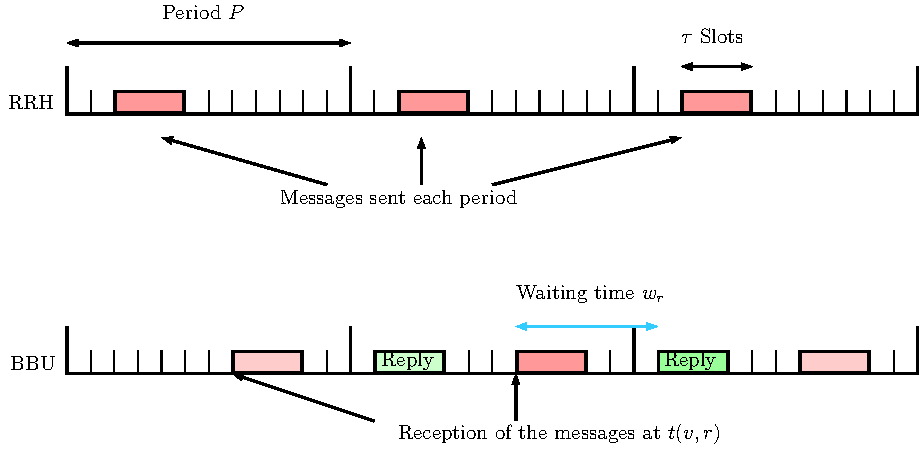
\includegraphics[width=0.47\textwidth]{rrh.pdf}
      \end{center}
      \caption{Periodic process}
      \end{figure}
      
%          Note that, in the process we describe, we do not take into account time the computation time a BBU needs to deal with one message. It can be encoded in the weight of the last arc leading to the BBU and thus we do not need to consider it explicitly in our model. 
The process time for a message sent on the route $r$ is equal to $PT(r)=\lambda(r)+ w_r+\lambda(r)$. Each route must respect some time limit that we call a \emph{deadline}. To represent these deadlines, 
      we use a deadline function $d$, which maps to each route $r$ an integer such that $PT(r)$ must be less than $d(r)$.
    We can now define the problem we solve in this article.

      \noindent {\bf Periodic Assignment for Low Latency (\pall)} 

 
      \noindent {\bf Input:}  A symmetric routed network $(G,{\cal R})$, the integers $P$, $\tau$ and a deadline function $d$.
      
      \noindent {\bf Question:} does there exist a $(P,\tau)$-periodic assignment $m$ of $(G,{\cal R})$ such that for all $r \in {\cal R}$, $PT(r) \leq d(r)$?



      It turns out that the problem \pall is $\NP$-hard to solve and even to approximate for \emph{general} routed networks (see the long version \cite{versionlongue}).      
        We also consider a simpler version of \pall, that we call {\bf Periodic Assignment for Zero Latency} or \pazl: we ask for a $(P,\tau)$-periodic assignment {\bf with all waiting times equal to $0$}. We introduce \pazl because it is simpler to study and we are able to prove theoretical results and find better algorithms than for \pall. As we  experimentally show in Sec.~\ref{sec:exp_PAZL}, this problem can often be solved positively albeit less often than the general problem. Finally, a solution to \pazl is simpler to implement in real telecommunication networks, since we do not need buffering at all. 
       
    
    \subsection{The star routed network}
    
     Let us define a family of simple routed networks modeling a Point-to-Multipoint fronthaul (PtMP), which has been designed for C-RAN \cite{tayq2017real}. 
      The graph $G$ has two sets of vertices, $S=\{s_0,...,s_{n-1}\}$ and $T=\{t_0,...,t_{n-1}\}$ of cardinality $n$ and two special nodes:
      the central source node {\bf $c_s$} and the central target node {\bf $c_t$}.
      There is an arc between {\bf $c_s$} and {\bf $c_t$} and for all $i$, there is an arc between $s_i$ and $c_s$ and between $t_i$ and $c_t$.
      All the symmetric arcs are also in the graph with the same weights.
      The forward routes are the directed paths $r_i = (s_i,c_s,c_t,t_i)$ and $\rho(r_i) = (t_i,c_t,c_s,s_i)$ which define a symmetric routed network. 
      The symmetric routed networks $(G, \{r_i,\rho(r_i)\}_{i<n})$ is called a \textbf{star routed network}. This graph looks very simple, but every network in which all routes share an arc can be reduced to a star routed network. This topology is realistic, since often all the BBUs are located in the same data-center. 
      In the following we will consider the problems \pall and \pazl on star routed networks only. 
      In this context, we can assume w.l.o.g. that the weights are zero on $(c_s,c_t)$ and for all $i$ on $(s_i,c_s)$ (see~\cite{versionlongue}).

%In such a situation, we can see the weights of the arcs $(c_t,t_i)$ either as all equals (in that case, the problem is trivial, see Sec.\ref{sec:PALL}) or different due to the structure of the network inside the data-center and the various hardwares used for different BBUs. 
%      
%      \todo{Dire ce qu'on peut supposer sur le star routed network}
      
%      \begin{figure}
%       \begin{center}
%	 \scalebox{0.8}{
%\begin{tikzpicture}
%
%\tikzset{EdgeStyle/.style={<->,font=\scriptsize,above,sloped,midway}}
%  \SetGraphUnit{5}
%  
%  \node[draw,circle] (s3) at (0, 0) {$s_2$}; 
%  \node[draw,circle] (s2) at (0, 2) {$s_1$}; 
%  \node[draw,circle] (s1) at (0, 4) {$s_0$}; 
%
%  \node[draw,circle] (t3) at (8, 0) {$t_2$}; 
%  \node[draw,circle] (t2) at (8, 2) {$t_1$}; 
%  \node[draw,circle] (t1) at (8, 4) {$t_0$}; 
%  
%
%  \node[draw,circle] (cs) at (3, 2) {$c_s$}; 
%  \node[draw,circle] (ct) at (5, 2) {$c_t$}; 
%
%  
%  \Edge[label = $\omega(s_1\,c_s)$](s1)(cs)
%  \Edge[label = $\omega(...)$](s2)(cs)
%  \Edge[label = $\omega(...)$](s3)(cs)
%  
%  \Edge[label = $\omega(...)$](ct)(t1)
%  \Edge[label = $\omega(...)$](ct)(t2)
%  \Edge[label = $\omega(...)$](ct)(t3)
%  
%  \Edge(cs)(ct)
%
%  
%\end{tikzpicture}
%}
%
%  \end{center}
%  \caption{A star routed network}
%  \end{figure}
% 	
%   Since the central arc appears in every route, its value does not matter when considering the process time of an assignment.
%   Moreover an assignment without collisions is also an assignment without collisions of the same star routed network with the weight of the central arc set to $0$. Hence, we assume from now on that the weight of the central arc is $0$.
%       
%       
%   Collisions between messages can only appear on the arc $(c_s,c_t)$ between forward routes or on the arc $(c_t,c_s)$
%   between backward routes. The flow of messages in a star routed network is completely described by their repartition in two time windows of size $P$, the {\bf forward period} which contains all $[t(c_s,r)]$ with $r$ a forward route and the {\bf backward period} which contains all $[t(c_t,r)]$ with $r$ a backward route.


\section{The Star Routed Network: No Waiting Time} \label{sec:PAZL}
  
  
     In this section, we deal with the problem PAZL on star routed networks. We want an assignment with waiting times zero, that is, $d(r) = 2\lambda(r)$ . For a route $r$, choosing the offset $m_r$ also sets the offset of the route $\rho(r)$ to $m_{\rho(r)} = m_{r} + \lambda(r) \mod P$.

    \subsection{Three algorithms to solve \pazl}

    We first present a simple policy, which works when the period is large with regard to the lengths of the routes.
    The messages are sent in order from the shortest route to the longest route, without any gap between two messages in the forward period.
    In other words, we assume that the route $r_i$ are sorted by increasing $\lambda(r_i)$ and we set $m_{r_i}$ the offset of $r_i$ to $i\tau$. We call this algorithm {\bf Shortest-Longest}.
    
      \begin{proposition} Let $(G, {\cal R})$ be a star routed network, and let $n\tau + 2(\lambda(r_{n-1}) - \lambda(r_{0})) \leq P$. There is a $(P,\tau)$-periodic assignment of $(G, {\cal R})$ with waiting times $0$ given by Shortest-Longest in time $O(n\log(n))$.\label{prop:SL}
      \end{proposition}

      
%     By definition, there are no collisions in the forward period and if the period is long enough, 
%     it is easy to see that in the backward period the order of the messages are the same as in the forward period and that no collision can occur. On the full version of this paper, one can found the proof that this algorithm always gives a solution if  $n\tau + 2(\lambda(r_{n-1}) - \lambda(r_{0})) \leq P$.

      We define the \textbf{load} of a star routed network as $\frac{n\tau}{P}$, it is the proportion of time slots used by messages on the central arc in a period. Therefore if the load is larger than $1$ there cannot be an assignment. We propose a greedy algorithm to build a $(P,\tau)$-periodic assignment. We consider the forward period and cut it into consecutive intervals of size $\tau$ that we call macro-slots. The algorithm works by choosing an offset for each route in the following way: try all offsets which put the message in a yet not used macro-slot in the forward  period. Since the choice of an offset also sets the position of the message in the backward period, chose the first one which does not create a collision. This algorithm always finds an assignment when the load is sufficiently large, since it guarantees that enough macro-slots are free.
      
      \begin{proposition}
    There is a $(P,\tau)$-periodic assignment of a star routed network with waiting times $0$ if the load is less than $1/3$ and it can be found in time $O(n^2)$.
    \end{proposition}
    
Finally, there is an algorithm which finds an assignment when it exists, in fixed parameter tractable time ($\FPT$) with parameter $n$ the number of routes, that is the algorithm is exponential in $n$ only and linear in the other parameters. This is justified since $n$ is small in practice (from $10$ to $20$) and the other parameters such as $P$, $\tau$ or the weights are large. We call this algorithm \textbf{Exhaustive Search of Compact Assignments}. The algorithm is based on a canonical form for assignments with waiting time zero, which allows to enumerate them in reasonable time. To make it more efficient in practice, we make cuts in the search tree used to explore all canonical assignments. 

   \subsection{Experimental evaluation}\label{sec:exp_PAZL}
   
   In this section we compare the three presented algorithms experimentally. From the C-RAN context we choose the following parameters: the number of routes is at most $n = 20$, $\tau$ is equal to $2,500$. It corresponds to slots of $64$ bits, messages of approximately $1$Mb and links of bandwidth $10$Gbps when $P$ is one millisecond.       
      First we consider routes which are shorter than $\tau$: a message cannot be contained completely in a single arc which is common in our applications. We generate star routed networks with weights of the arcs $(c_t,t_i)$ drawn uniformly between $0$ and $700$ which corresponds to links of less than $5$km between a BBU and an RRH. 

        
      \begin{figure}[h]
      \begin{center}
	 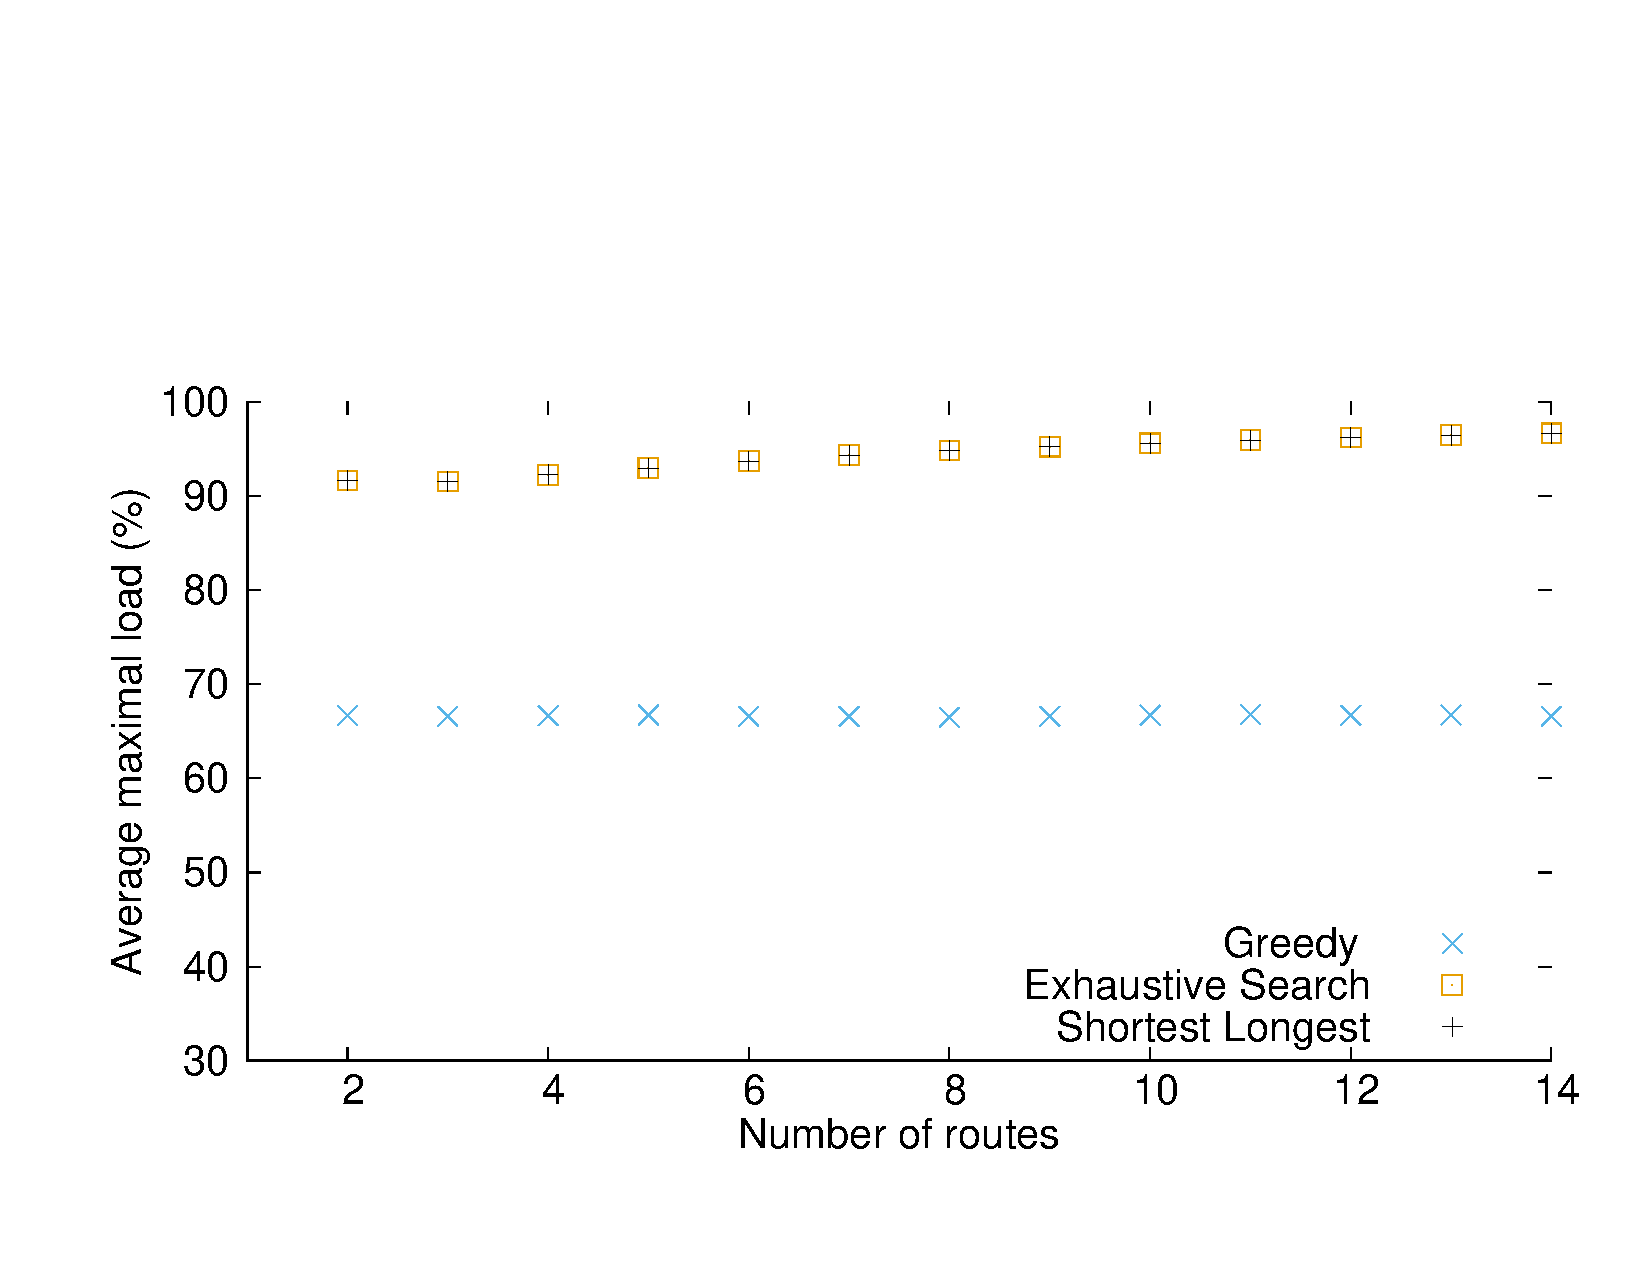
\includegraphics[width=0.47\textwidth]{periode_petite.pdf}
      \end{center}
      \caption{Maximal load averaged over $1,000$ random instances}\label{fig:short}
      \end{figure}
      
      
      For short routes, both  Shortest Longest or the exhaustive search have the same performance and succeed very often but \emph{not always}. It is surprising, since exhaustive search is guaranteed to find a solution when it exists, while Shortest Longest is only an heuristic. The Greedy algorithm is less effective but it works when the load is less than $0.6$, much better than the theoritical bound of $1/3$. We now look at the performance of the algorithms on longer routes. The weights of the arcs are drawn between $0$ and $20,000$.

   
\begin{figure}[h]

       \begin{center}
      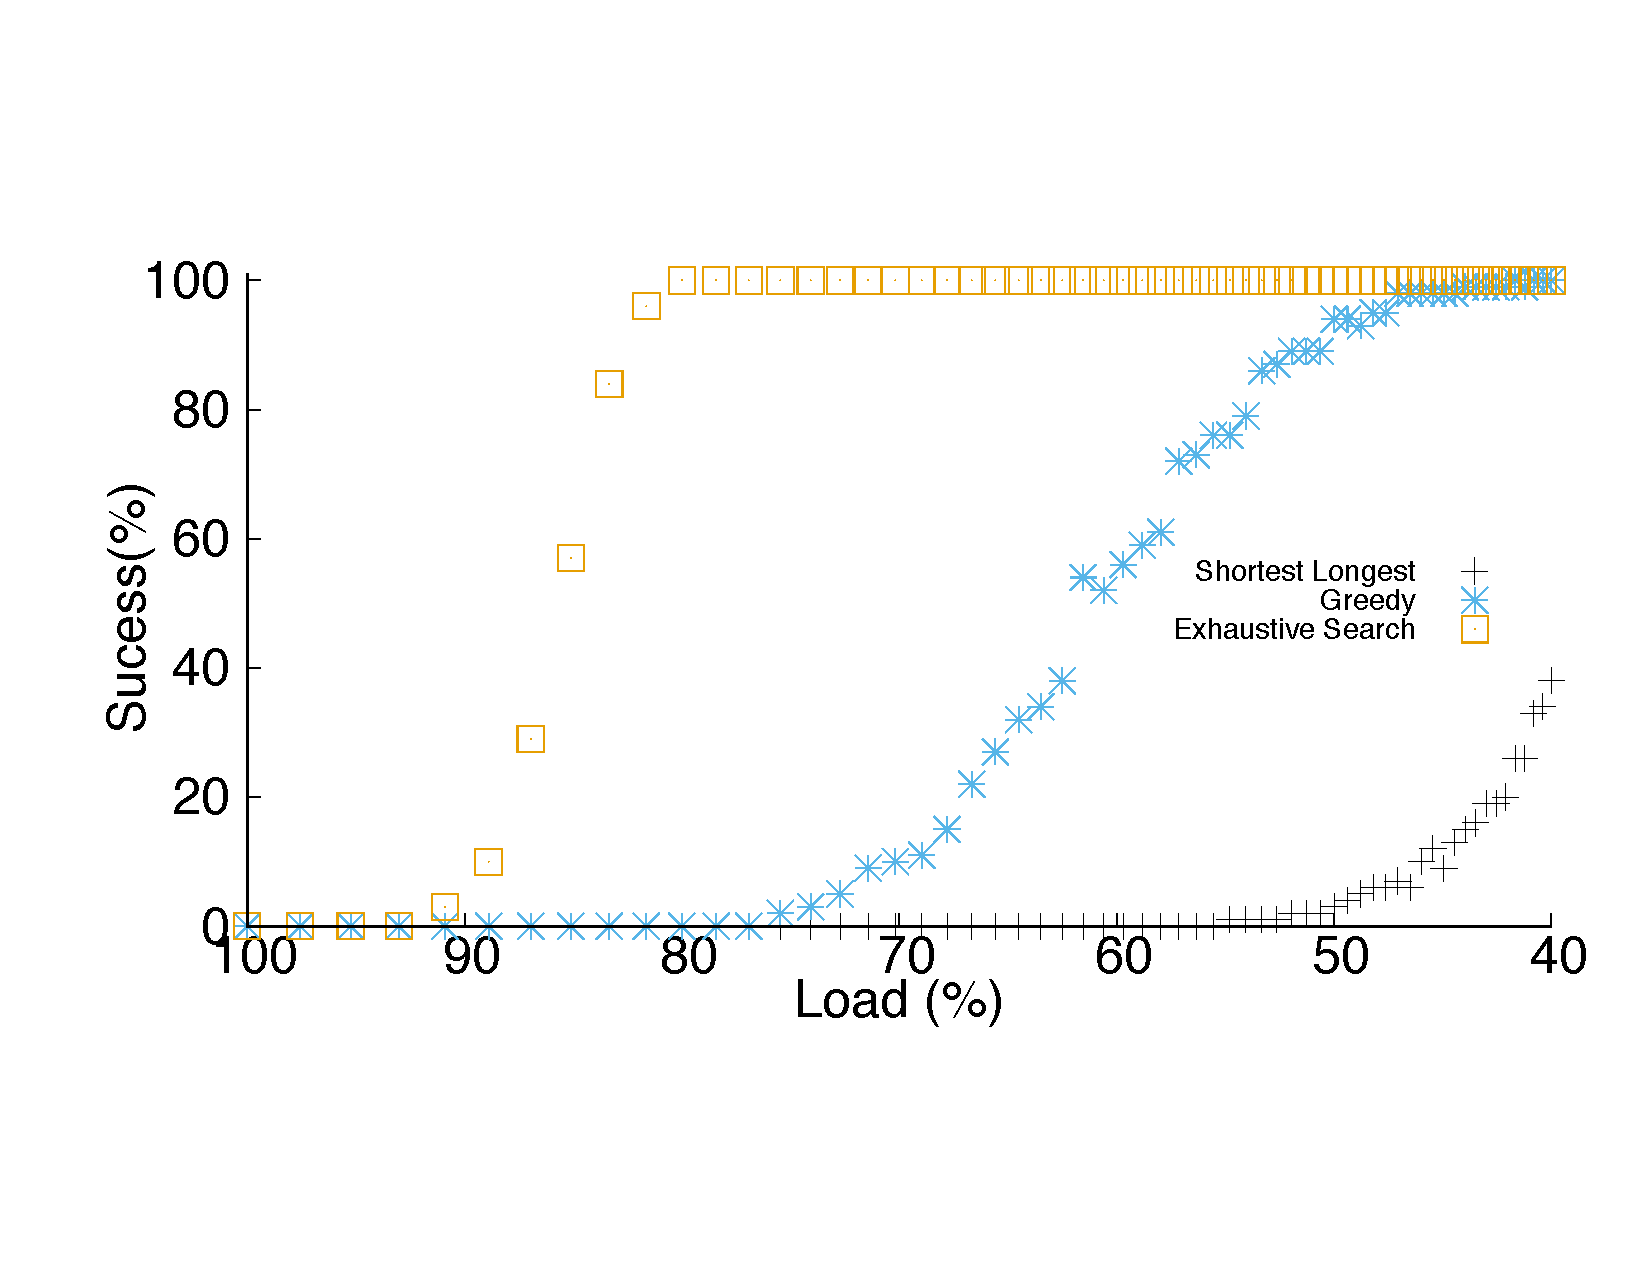
\includegraphics[width=0.47\textwidth]{echec_longues.pdf}
      \end{center}
       
      \caption{Success rate for $8$ routes over $1,000$ random instances}\label{fig:long}
     \end{figure}
     
     On long routes, the performances of Shortest-Longest are abysmal since the difference between the length of the routes is large.
       When the load is larger than $50\%$, the exhaustive search finds more solutions than the greedy algorithms which justifies its use. However, for load larger than $80\%$ there are many instances for which there are no solutions to \pazl.
        It means that with long routes and high load, looking for an assignment without waiting time is far too restrictive. That is why we present algorithms for the general \pall problem in our next section. 
     

         \section{Solving \pall on Star Routed Networks}\label{sec:PALL}
         
    In this section, we consider the more general \pall problem on star routed networks. The messages are allowed to wait in the target vertices (BBUs) to yield more possible assignments. Hence, we allow the process time of a route to be greater than twice the weights of the route, but it is bounded by its deadline.
  
  \subsection{Two algorithms to solve \pazl}
  
  As for \pazl, it is possible to design an FPT algorithm for \pall~\cite{versionlongue}. 
  However, it is complicated and its running time is too large even for small $n$,
  thus we do not describe it here or test it against the two other algorithms we present.
  
  In the two following algorithms, we assume that the offsets of the forward routes are already fixed by some mechanism, hence they fix only the offsets of the backward routes. 
    
    The first algorithm we propose to solve \pall is a greedy algorithm which sets the offset $m_{\rho(r_i)}$ of the 
    backward routes. It prioritizes the routes with the earliest deadline to best satisfy the
    constraint on the process time. We call it \textbf{Greedy Deadline (GD)}. We say that a backward route $\rho(r_i)$ is {\bf eligible} at time $t$ if the message of the route $\rho(r_i)$ arrives at $c_t$ before time $t$ with $w_i = 0$. For each time $t$, amongst all eligible routes at $t$, we choose the one with the smallest deadline and fix its offset to $t$.
    This algorithm can fail since it does not take into account the periodicity.
    
     The problem \pall is very similar to the following scheduling problem. Given a set of jobs with \emph{release times} and  \emph{deadlines}, schedule all jobs on a single processor, that is choose the time at which they are computed, so that no two jobs are scheduled at the same time. When the running time is the same on all jobs, this problem can be solved in polynomial time~\cite{simons1978fast}. We use the polynomial time scheduling algorithm to solve \pall and we make some adjustments to take the periodicity into account: we run it once for each forward route $r$ and we fix $m_r$ so that the waiting time for this route is zero and we change the deadline of each route $r'$ to be less than $m_{r} + P$. The algorithm we obtain, when it succeeds always finds a correct peridoic assignment and we call it {\bf Periodic Minimal Latency Scheduling (PMLS)}.

     
    \subsection{Experimental evaluation}
    \label{sec:resultsPALL}
    
    We set the number of routes to $8$ to make comparisons with the results of Section~\ref{sec:exp_PAZL} easier. 
    We draw uniformly the weights of the arcs between $0$ and $20,000$. We consider load of $95\%$, since for small load solving \pazl is enough as shown in Section~\ref{sec:exp_PAZL}. To simplify the experiments, 
    we use \emph{the same deadline} for all routes. We define the {\bf margin} as the difference between the deadline and twice the longest route. The margin represents the latency imposed by the communication process without taking into account the physical length of the network which cannot be changed.
  
   
   To set the offsets of the forward routes, we draw random orders on these routes, so that their messages goes through 
   the central arc in this order. If we have $n$ routes and draw the order given by the permutation $\sigma$ then we set $m_{i} = \sigma(i)\tau$. In the experiments, we draw $1000$ random orders and consider that the algorithm fixing the offsets of the backward routes succeds when it succeeds for one of the random orders.
      
     
    \begin{figure} 
       \begin{center}
      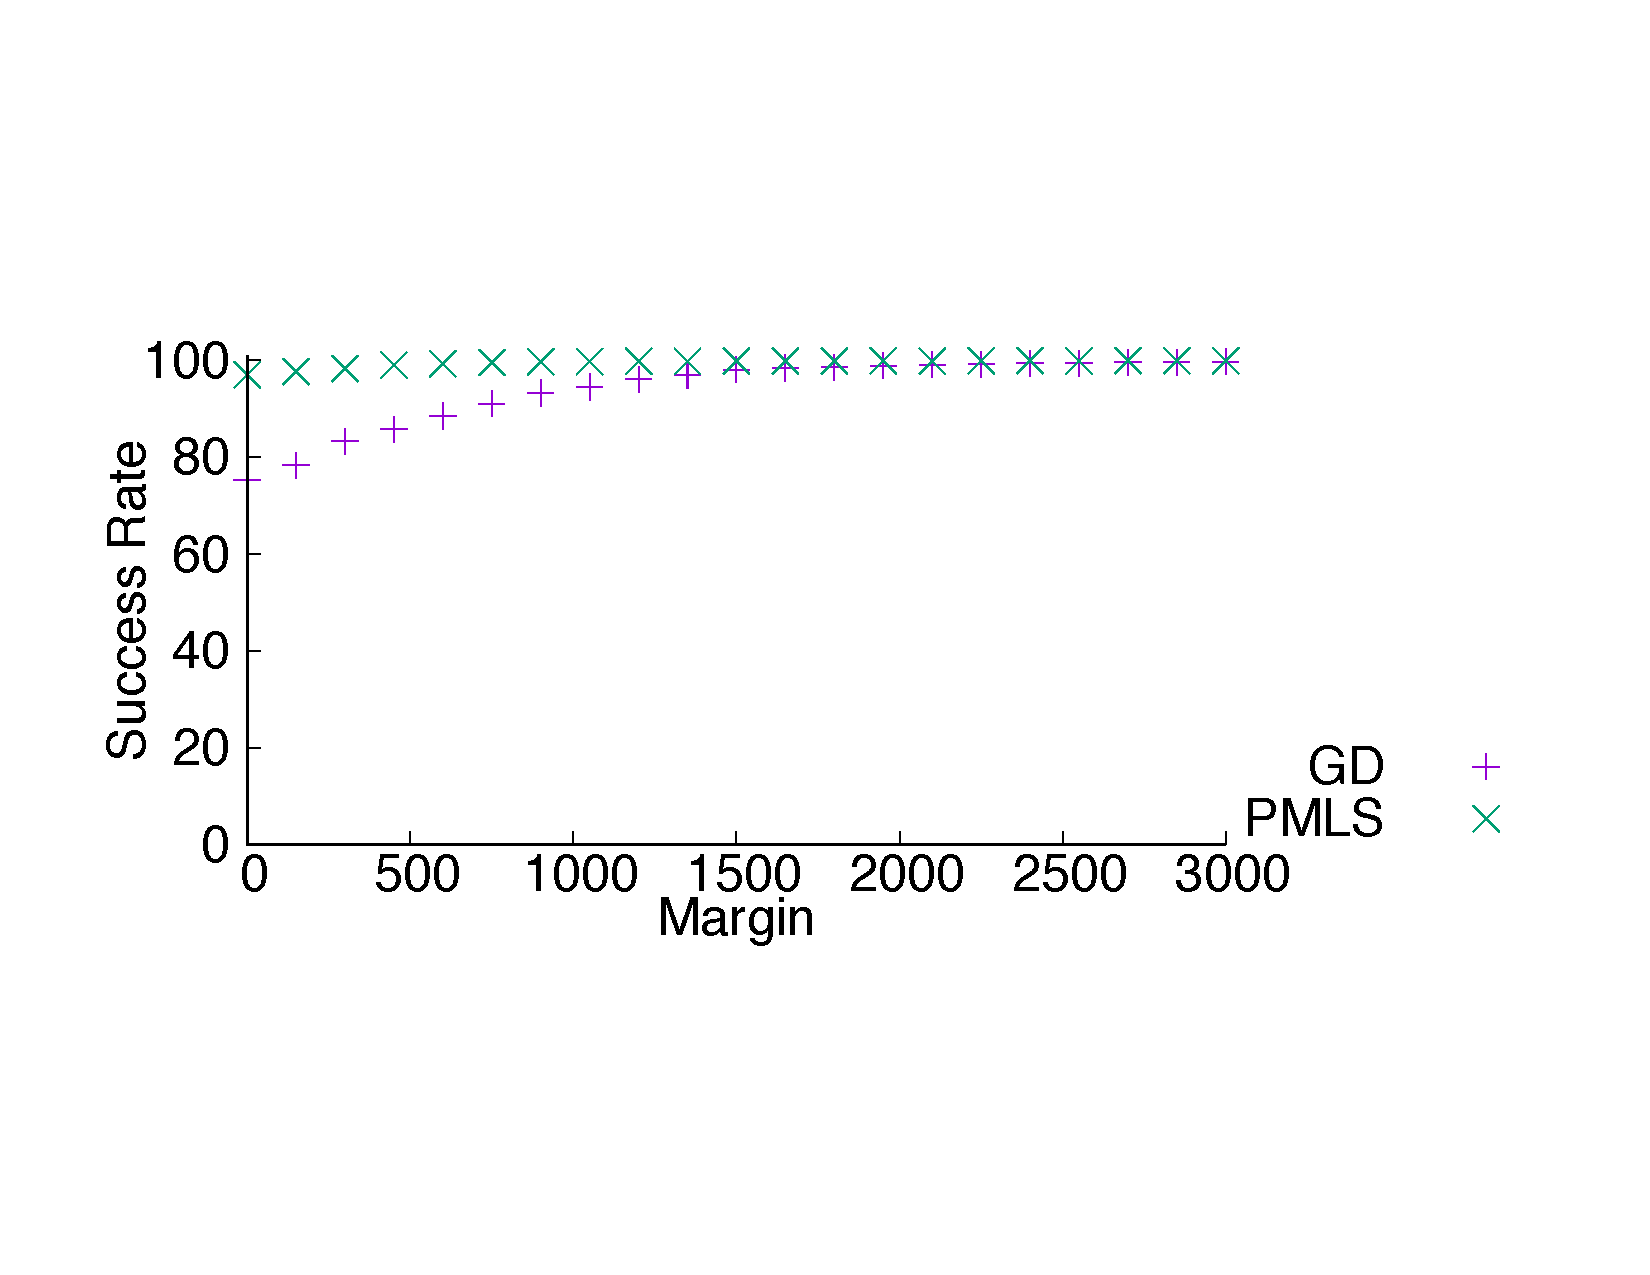
\includegraphics[width=0.5\textwidth]{retour_21000.pdf}
      \end{center}
      \caption{Success rate of GD and PMLS, over $10,000$ instances, $95\%$ load}
     \label{fig:success21000}
    
     \end{figure}
        
     
Fig.~\ref{fig:success21000} shows that PMLS is better than GD since it finds a solution in more than $97\%$ of the experiments, even with a margin $0$. Therefore, for the worst possible constraints on load and margin, there are a few instances for which we do not find a solution. With a margin of $1,000$, which corresponds to about $0.05$ms of additional delay with the chosen parameters, we always find a solution. The success rate of these algorithms depends on the number of random orders drawn to fix the offsets of forward routes. It turns out that PMLS needs much less random orders than GD to work well, which makes it even better than GD.   


    We now compare the performances of our algorithms to find periodic assignments against the actual way to manage the messages in a network:  statistical multiplexing with a FIFO buffer in each node of the network to resolve collisions. The time at which the messages are sent in the network is not computed as in our approach, thus we fix the offsets of each route to some random value.
     Even if this policy seems to work in practice when the network is not too loaded, it does not give any guarantee on the latency. Remark that the process is not periodic, therefore we must measure the process time of each route over several periods if we want to compute its maximum. We choose to simulate it for $1,000$ periods and we have observed that the process time usually stabilizes after $10$ periods. The margin is defined as the maximum process time, computed as explained, minus twice the size of the longest route. 
	    
     In Figure.~\ref{fig:sto}, we represent the probability of success for statistical multiplexing and PMLS for different margin. The distribution is computed from $1000$ star routed networks drawn with the same parameters as before. We represent the distribution under high and light load for statistical multiplexing and under high load only for PMLS since under light load the margin is always $0$. 
     

    \begin{figure}
       \begin{center}
      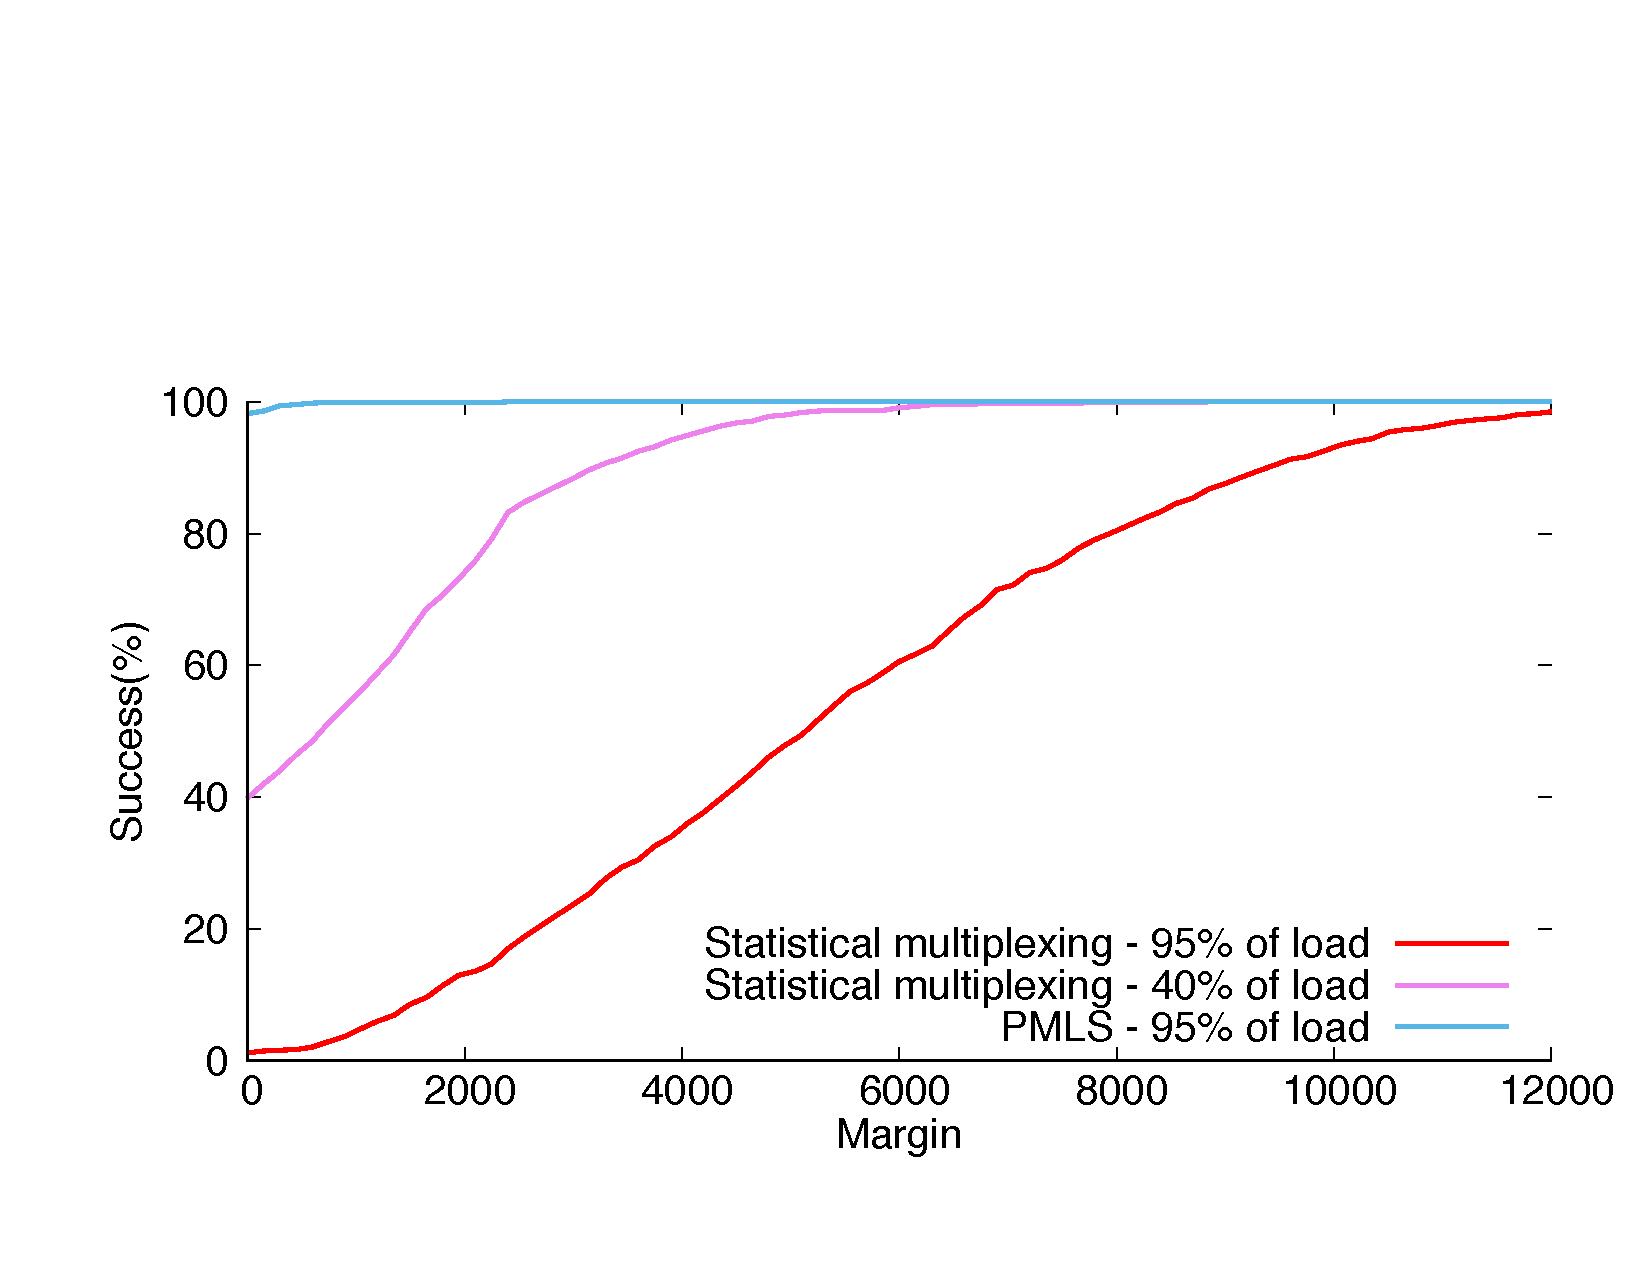
\includegraphics[width = 0.45\textwidth]{stochastic.pdf}
       %% GNUPLOT: LaTeX picture
\setlength{\unitlength}{0.240900pt}
\ifx\plotpoint\undefined\newsavebox{\plotpoint}\fi
\sbox{\plotpoint}{\rule[-0.200pt]{0.400pt}{0.400pt}}%
\begin{picture}(1500,900)(0,0)
\sbox{\plotpoint}{\rule[-0.200pt]{0.400pt}{0.400pt}}%
\put(171.0,131.0){\rule[-0.200pt]{4.818pt}{0.400pt}}
\put(151,131){\makebox(0,0)[r]{$0$}}
\put(1279.0,131.0){\rule[-0.200pt]{4.818pt}{0.400pt}}
\put(171.0,212.0){\rule[-0.200pt]{4.818pt}{0.400pt}}
\put(151,212){\makebox(0,0)[r]{$1000$}}
\put(1279.0,212.0){\rule[-0.200pt]{4.818pt}{0.400pt}}
\put(171.0,293.0){\rule[-0.200pt]{4.818pt}{0.400pt}}
\put(151,293){\makebox(0,0)[r]{$2000$}}
\put(1279.0,293.0){\rule[-0.200pt]{4.818pt}{0.400pt}}
\put(171.0,374.0){\rule[-0.200pt]{4.818pt}{0.400pt}}
\put(151,374){\makebox(0,0)[r]{$3000$}}
\put(1279.0,374.0){\rule[-0.200pt]{4.818pt}{0.400pt}}
\put(171.0,455.0){\rule[-0.200pt]{4.818pt}{0.400pt}}
\put(151,455){\makebox(0,0)[r]{$4000$}}
\put(1279.0,455.0){\rule[-0.200pt]{4.818pt}{0.400pt}}
\put(171.0,535.0){\rule[-0.200pt]{4.818pt}{0.400pt}}
\put(151,535){\makebox(0,0)[r]{$5000$}}
\put(1279.0,535.0){\rule[-0.200pt]{4.818pt}{0.400pt}}
\put(171.0,616.0){\rule[-0.200pt]{4.818pt}{0.400pt}}
\put(151,616){\makebox(0,0)[r]{$6000$}}
\put(1279.0,616.0){\rule[-0.200pt]{4.818pt}{0.400pt}}
\put(171.0,697.0){\rule[-0.200pt]{4.818pt}{0.400pt}}
\put(151,697){\makebox(0,0)[r]{$7000$}}
\put(1279.0,697.0){\rule[-0.200pt]{4.818pt}{0.400pt}}
\put(171.0,778.0){\rule[-0.200pt]{4.818pt}{0.400pt}}
\put(151,778){\makebox(0,0)[r]{$8000$}}
\put(1279.0,778.0){\rule[-0.200pt]{4.818pt}{0.400pt}}
\put(171.0,859.0){\rule[-0.200pt]{4.818pt}{0.400pt}}
\put(151,859){\makebox(0,0)[r]{$9000$}}
\put(1279.0,859.0){\rule[-0.200pt]{4.818pt}{0.400pt}}
\put(171.0,131.0){\rule[-0.200pt]{0.400pt}{4.818pt}}
\put(171,90){\makebox(0,0){$20000$}}
\put(171.0,839.0){\rule[-0.200pt]{0.400pt}{4.818pt}}
\put(359.0,131.0){\rule[-0.200pt]{0.400pt}{4.818pt}}
\put(359,90){\makebox(0,0){$25000$}}
\put(359.0,839.0){\rule[-0.200pt]{0.400pt}{4.818pt}}
\put(547.0,131.0){\rule[-0.200pt]{0.400pt}{4.818pt}}
\put(547,90){\makebox(0,0){$30000$}}
\put(547.0,839.0){\rule[-0.200pt]{0.400pt}{4.818pt}}
\put(735.0,131.0){\rule[-0.200pt]{0.400pt}{4.818pt}}
\put(735,90){\makebox(0,0){$35000$}}
\put(735.0,839.0){\rule[-0.200pt]{0.400pt}{4.818pt}}
\put(923.0,131.0){\rule[-0.200pt]{0.400pt}{4.818pt}}
\put(923,90){\makebox(0,0){$40000$}}
\put(923.0,839.0){\rule[-0.200pt]{0.400pt}{4.818pt}}
\put(1111.0,131.0){\rule[-0.200pt]{0.400pt}{4.818pt}}
\put(1111,90){\makebox(0,0){$45000$}}
\put(1111.0,839.0){\rule[-0.200pt]{0.400pt}{4.818pt}}
\put(1299.0,131.0){\rule[-0.200pt]{0.400pt}{4.818pt}}
\put(1299,90){\makebox(0,0){$50000$}}
\put(1299.0,839.0){\rule[-0.200pt]{0.400pt}{4.818pt}}
\put(171.0,131.0){\rule[-0.200pt]{0.400pt}{175.375pt}}
\put(171.0,131.0){\rule[-0.200pt]{271.735pt}{0.400pt}}
\put(30,495){\makebox(0,0){Needed Flexibility}}
\put(735,29){\makebox(0,0){Period}}
\put(171.0,455.0){\rule[-0.200pt]{0.400pt}{81.183pt}}
\put(171.0,455.0){\rule[-0.200pt]{2.409pt}{0.400pt}}
\put(171.0,792.0){\rule[-0.200pt]{2.409pt}{0.400pt}}
\put(209.0,412.0){\rule[-0.200pt]{0.400pt}{73.715pt}}
\put(199.0,412.0){\rule[-0.200pt]{4.818pt}{0.400pt}}
\put(199.0,718.0){\rule[-0.200pt]{4.818pt}{0.400pt}}
\put(246.0,353.0){\rule[-0.200pt]{0.400pt}{79.497pt}}
\put(236.0,353.0){\rule[-0.200pt]{4.818pt}{0.400pt}}
\put(236.0,683.0){\rule[-0.200pt]{4.818pt}{0.400pt}}
\put(284.0,336.0){\rule[-0.200pt]{0.400pt}{75.883pt}}
\put(274.0,336.0){\rule[-0.200pt]{4.818pt}{0.400pt}}
\put(274.0,651.0){\rule[-0.200pt]{4.818pt}{0.400pt}}
\put(321.0,306.0){\rule[-0.200pt]{0.400pt}{70.343pt}}
\put(311.0,306.0){\rule[-0.200pt]{4.818pt}{0.400pt}}
\put(311.0,598.0){\rule[-0.200pt]{4.818pt}{0.400pt}}
\put(359.0,297.0){\rule[-0.200pt]{0.400pt}{73.715pt}}
\put(349.0,297.0){\rule[-0.200pt]{4.818pt}{0.400pt}}
\put(349.0,603.0){\rule[-0.200pt]{4.818pt}{0.400pt}}
\put(397.0,270.0){\rule[-0.200pt]{0.400pt}{63.598pt}}
\put(387.0,270.0){\rule[-0.200pt]{4.818pt}{0.400pt}}
\put(387.0,534.0){\rule[-0.200pt]{4.818pt}{0.400pt}}
\put(434.0,269.0){\rule[-0.200pt]{0.400pt}{64.561pt}}
\put(424.0,269.0){\rule[-0.200pt]{4.818pt}{0.400pt}}
\put(424.0,537.0){\rule[-0.200pt]{4.818pt}{0.400pt}}
\put(472.0,238.0){\rule[-0.200pt]{0.400pt}{69.138pt}}
\put(462.0,238.0){\rule[-0.200pt]{4.818pt}{0.400pt}}
\put(462.0,525.0){\rule[-0.200pt]{4.818pt}{0.400pt}}
\put(509.0,226.0){\rule[-0.200pt]{0.400pt}{62.393pt}}
\put(499.0,226.0){\rule[-0.200pt]{4.818pt}{0.400pt}}
\put(499.0,485.0){\rule[-0.200pt]{4.818pt}{0.400pt}}
\put(547.0,222.0){\rule[-0.200pt]{0.400pt}{60.225pt}}
\put(537.0,222.0){\rule[-0.200pt]{4.818pt}{0.400pt}}
\put(537.0,472.0){\rule[-0.200pt]{4.818pt}{0.400pt}}
\put(585.0,195.0){\rule[-0.200pt]{0.400pt}{60.225pt}}
\put(575.0,195.0){\rule[-0.200pt]{4.818pt}{0.400pt}}
\put(575.0,445.0){\rule[-0.200pt]{4.818pt}{0.400pt}}
\put(622.0,185.0){\rule[-0.200pt]{0.400pt}{58.780pt}}
\put(612.0,185.0){\rule[-0.200pt]{4.818pt}{0.400pt}}
\put(612.0,429.0){\rule[-0.200pt]{4.818pt}{0.400pt}}
\put(660.0,178.0){\rule[-0.200pt]{0.400pt}{59.743pt}}
\put(650.0,178.0){\rule[-0.200pt]{4.818pt}{0.400pt}}
\put(650.0,426.0){\rule[-0.200pt]{4.818pt}{0.400pt}}
\put(697.0,188.0){\rule[-0.200pt]{0.400pt}{59.020pt}}
\put(687.0,188.0){\rule[-0.200pt]{4.818pt}{0.400pt}}
\put(687.0,433.0){\rule[-0.200pt]{4.818pt}{0.400pt}}
\put(735.0,152.0){\rule[-0.200pt]{0.400pt}{55.889pt}}
\put(725.0,152.0){\rule[-0.200pt]{4.818pt}{0.400pt}}
\put(725.0,384.0){\rule[-0.200pt]{4.818pt}{0.400pt}}
\put(773.0,146.0){\rule[-0.200pt]{0.400pt}{57.575pt}}
\put(763.0,146.0){\rule[-0.200pt]{4.818pt}{0.400pt}}
\put(763.0,385.0){\rule[-0.200pt]{4.818pt}{0.400pt}}
\put(810.0,146.0){\rule[-0.200pt]{0.400pt}{54.925pt}}
\put(800.0,146.0){\rule[-0.200pt]{4.818pt}{0.400pt}}
\put(800.0,374.0){\rule[-0.200pt]{4.818pt}{0.400pt}}
\put(848.0,143.0){\rule[-0.200pt]{0.400pt}{56.371pt}}
\put(838.0,143.0){\rule[-0.200pt]{4.818pt}{0.400pt}}
\put(838.0,377.0){\rule[-0.200pt]{4.818pt}{0.400pt}}
\put(885.0,140.0){\rule[-0.200pt]{0.400pt}{56.371pt}}
\put(875.0,140.0){\rule[-0.200pt]{4.818pt}{0.400pt}}
\put(875.0,374.0){\rule[-0.200pt]{4.818pt}{0.400pt}}
\put(923.0,133.0){\rule[-0.200pt]{0.400pt}{54.202pt}}
\put(913.0,133.0){\rule[-0.200pt]{4.818pt}{0.400pt}}
\put(913.0,358.0){\rule[-0.200pt]{4.818pt}{0.400pt}}
\put(961.0,131.0){\rule[-0.200pt]{0.400pt}{55.166pt}}
\put(951.0,131.0){\rule[-0.200pt]{4.818pt}{0.400pt}}
\put(951.0,360.0){\rule[-0.200pt]{4.818pt}{0.400pt}}
\put(998.0,131.0){\rule[-0.200pt]{0.400pt}{49.384pt}}
\put(988.0,131.0){\rule[-0.200pt]{4.818pt}{0.400pt}}
\put(988.0,336.0){\rule[-0.200pt]{4.818pt}{0.400pt}}
\put(1036.0,131.0){\rule[-0.200pt]{0.400pt}{48.180pt}}
\put(1026.0,131.0){\rule[-0.200pt]{4.818pt}{0.400pt}}
\put(1026.0,331.0){\rule[-0.200pt]{4.818pt}{0.400pt}}
\put(1073.0,131.0){\rule[-0.200pt]{0.400pt}{47.216pt}}
\put(1063.0,131.0){\rule[-0.200pt]{4.818pt}{0.400pt}}
\put(1063.0,327.0){\rule[-0.200pt]{4.818pt}{0.400pt}}
\put(1111.0,131.0){\rule[-0.200pt]{0.400pt}{46.975pt}}
\put(1101.0,131.0){\rule[-0.200pt]{4.818pt}{0.400pt}}
\put(1101.0,326.0){\rule[-0.200pt]{4.818pt}{0.400pt}}
\put(1149.0,131.0){\rule[-0.200pt]{0.400pt}{45.048pt}}
\put(1139.0,131.0){\rule[-0.200pt]{4.818pt}{0.400pt}}
\put(1139.0,318.0){\rule[-0.200pt]{4.818pt}{0.400pt}}
\put(1186.0,131.0){\rule[-0.200pt]{0.400pt}{46.494pt}}
\put(1176.0,131.0){\rule[-0.200pt]{4.818pt}{0.400pt}}
\put(1176.0,324.0){\rule[-0.200pt]{4.818pt}{0.400pt}}
\put(1224.0,131.0){\rule[-0.200pt]{0.400pt}{45.048pt}}
\put(1214.0,131.0){\rule[-0.200pt]{4.818pt}{0.400pt}}
\put(1214.0,318.0){\rule[-0.200pt]{4.818pt}{0.400pt}}
\put(1261.0,131.0){\rule[-0.200pt]{0.400pt}{41.194pt}}
\put(1251.0,131.0){\rule[-0.200pt]{4.818pt}{0.400pt}}
\put(171,608){\makebox(0,0){$+$}}
\put(209,562){\makebox(0,0){$+$}}
\put(246,503){\makebox(0,0){$+$}}
\put(284,479){\makebox(0,0){$+$}}
\put(321,431){\makebox(0,0){$+$}}
\put(359,429){\makebox(0,0){$+$}}
\put(397,390){\makebox(0,0){$+$}}
\put(434,382){\makebox(0,0){$+$}}
\put(472,367){\makebox(0,0){$+$}}
\put(509,340){\makebox(0,0){$+$}}
\put(547,327){\makebox(0,0){$+$}}
\put(585,317){\makebox(0,0){$+$}}
\put(622,307){\makebox(0,0){$+$}}
\put(660,302){\makebox(0,0){$+$}}
\put(697,300){\makebox(0,0){$+$}}
\put(735,278){\makebox(0,0){$+$}}
\put(773,273){\makebox(0,0){$+$}}
\put(810,268){\makebox(0,0){$+$}}
\put(848,267){\makebox(0,0){$+$}}
\put(885,254){\makebox(0,0){$+$}}
\put(923,248){\makebox(0,0){$+$}}
\put(961,259){\makebox(0,0){$+$}}
\put(998,234){\makebox(0,0){$+$}}
\put(1036,234){\makebox(0,0){$+$}}
\put(1073,232){\makebox(0,0){$+$}}
\put(1111,228){\makebox(0,0){$+$}}
\put(1149,216){\makebox(0,0){$+$}}
\put(1186,212){\makebox(0,0){$+$}}
\put(1224,227){\makebox(0,0){$+$}}
\put(1261,203){\makebox(0,0){$+$}}
\put(1251.0,302.0){\rule[-0.200pt]{4.818pt}{0.400pt}}
\put(171.0,131.0){\rule[-0.200pt]{0.400pt}{175.375pt}}
\put(171.0,131.0){\rule[-0.200pt]{271.735pt}{0.400pt}}
\end{picture}

      \end{center}
      \caption{Probability of success of statistical multiplexing and PMLS}
      \label{fig:sto}   
     \end{figure}    
 
     The experiment clearly shows that statistical multiplexing does not ensure a minimal latency. 
     The latency is extremely high when the load is high, with a margin of about $10,000$ for the worst $10\%$ which corresponds to half the period, that is $0.5$ms. Even when the network is lightly loaded, $20\%$ of the instances have a margin of more than $2,000$. On the other hand, PMLS finds an assignment with margin $0$ in a highly loaded network $97\%$ of the time! 

     For each $1000$ slots of latency we save from the periodic process, we are able to lengthen the routes of $10$km, which has a huge economical impact. We feel that it strongly justifies the use of a deterministic sending scheme for latency critical applications such as our C-RAN motivating problem.     
% 
%  \section{Conclusion}
% In this paper, we proposed two deterministic methods to establish a low latency periodic communication between BBUs and RRHs in 
% a star shaped fronthaul network. The first method uses no buffering and has no latency overhead. It works when the routes are short (Longest-Shortest policy) or when the load is less than $80\%$ (Exhaustive search of compact assignments).  
% When the load is higher, buffering is allowed in the BBUs and we propose the algorithm PMLS which  finds a deterministic communication scheme with almost no additional latency.
% 
%    
%    We plan to generalize our study of the \pall problem to other common fronthaul topologies,
% 
%    such as caterpillar, trees, cycles or bounded treewidth graphs. The cycles in particular are 
%    different since their forward and backward routes are not symmetric. 
%    We would like to design an FPT algorithm for \pall which is as efficient as the one for \pazl 
%    and prove that both problems are $\NP$-hard.
% 
%    We could also study variations of our problem. Instead of minimizing the maximum process time, we could try to minimize the average process time, a linear objective which could make linear programming useful. We could allow preemption, that is the messages are allowed to be cut into pieces, which would certainly change the complexity of the problem.  Instead of periodic communication we could try to organize communications with pseudo-periodic schemes or even a temporal law. Moreover we could allow a bounded message loss.
%    Finally, the routes may not be fixed but chosen in the graph to minimize the maximum process time, which would make the problem even more difficult (maybe $\Pi_2$-complete instead of $\NP$-complete). 

 \paragraph*{Acknowledgments} The authors thank Christian Cad\'er\'e and David Auger for the friendly discussions
 they had on the subject and their insightful remarks. This work is partially supported by the french ANR project N-GREEN.

\bibliographystyle{ieeetr}
\bibliography{Sources}

\end{document}
